\section{Quiz}

This remainder of this homework is a series of multiple choice questions related to the word2vec algorithm.

{\bf How to submit:}  Even though these are not coding questions, you will submit your response to
each question in the |src-quiz/submission.py| file.  This file will act as
your 'bubble sheet' for multiple choice questions in this course.  A sample response
might look like this:

\begin{center}
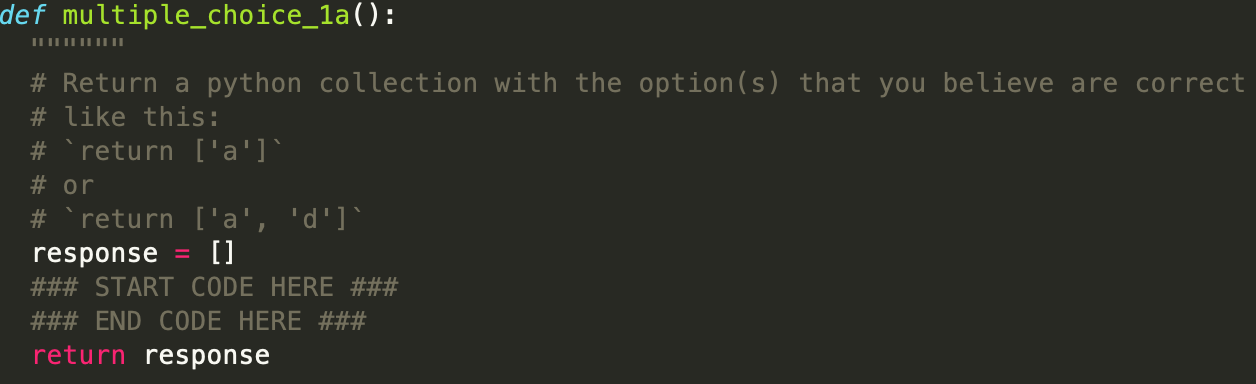
\includegraphics[width=1\textwidth]{sample_question_empty.png}
\end{center}

If you believe that |a| and |b| are the correct responses to this question, you
will type |response = [`a', `b']| between the indicated lines like this:

\begin{center}
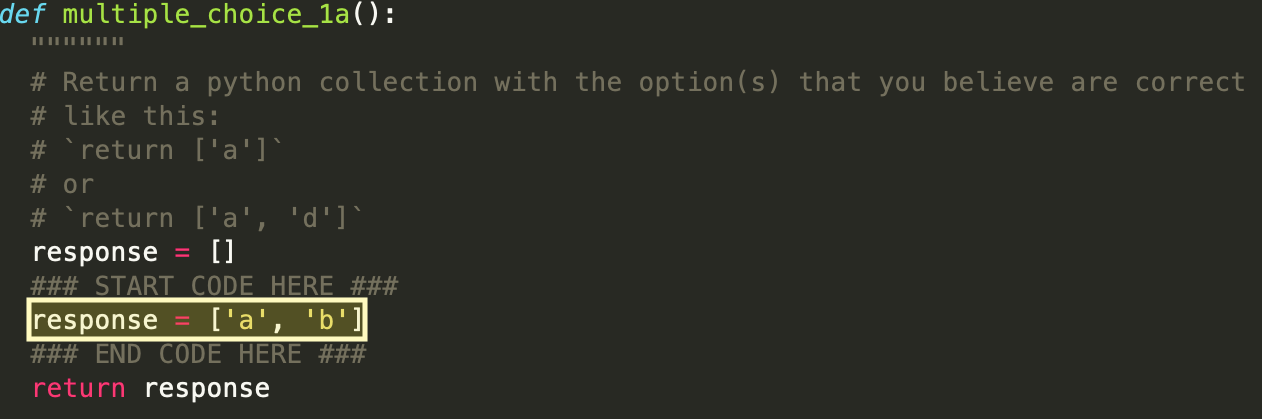
\includegraphics[width=1\textwidth]{sample_question_complete.png}
\end{center}

{\bf How to verify your submission:}
You can run the student version of the autograder locally like all coding
problem sets.  In the case of this problem set, the helper tests will verify
that your responses are within the set of possible choices for each question
(e.g. the helper functions will flag if you forget to answer a question of if
you respond with |[`a', `d']| when the choices are |[`a', `b', `c']|.)  See the
front pages of this assignment for instructions to run the autograder.
\clearpage

\begin{enumerate}[1.]
\item \points{quiz1}
Recall the standard Stochastic Gradient Descent update rule

\begin{equation*}
        \theta \gets \theta - \alpha \nabla_{\theta} J_{\text{minibatch}}(\theta)
\end{equation*}

where $\theta$ is a vector containing all of the model parameters, $J$ is the loss function, $\nabla_{\theta} J_{\text{minibatch}}(\theta)$ is the gradient of the loss function with respect to the parameters on a minibatch of data, and $\alpha$ is the learning rate.

Adam additionally uses a trick called momentum by keeping track of $m$, a rolling average of the gradients:
\begin{equation*}
    m \gets \beta_1m + (1 - \beta_1)\nabla_{\theta} J_{\text{minibatch}}(\theta)
\end{equation*}
        
\begin{equation*}
    \theta \gets \theta - \alpha m
\end{equation*}

where $\beta_1$ is a hyperparameter between 0 and 1 (often set to 0.9). This momentum trick helps in converging faster. Which of the following is true regarding the gradient update using momentum?

\begin{enumerate}[(a)]
\item Relative to SGD, each update will not vary as much (the current gradient receives only a $1 - \beta1$ scaled update). This helps maintain a smaller variance and helps in faster convergence to a local optimum.
\item Relative to SGD, each update has a larger variance. This helps in faster convergence to a local optimum.
\item Setting $\beta_1$ to a low value would lead to faster convergence to a local optimum, relative to SGD.
\end{enumerate}

% ### START CODE HERE ###
% ### END CODE HERE ###

\item \points{quiz2}
Adam uses adaptive learning rates by keeping track of $v$, a rolling average of the magnitudes of the gradient:
        
\begin{equation*}
    m \gets \beta_1m + (1 - \beta_1)\nabla_{\theta} J_{\text{minibatch}}(\theta)
\end{equation*}

\begin{equation*}
    v \gets \beta_2v + (1 - \beta_2) (\nabla_{\theta} J_{\text{minibatch}}(\theta) \odot \nabla_{\theta} J_{\text{minibatch}}(\theta)
\end{equation*}

\begin{equation*}
    \theta \gets \theta - \alpha \odot m / \sqrt{v}
\end{equation*}

where $\odot$ and $/$ denote element-wise multiplication and division (so $z\odot z$ is element-wise squaring) and $\beta_2$ is a hyperparameter between 0 and 1 (often set to  0.99). Since Adam divides the update by $\sqrt{v}$, which of the model parameters will get larger updates? 

\begin{enumerate}[(a)]
\item The parameters with the smaller gradients (on average) will get larger updates. This means that when the loss is more flat with respect to a parameter, that parameter will get a larger update, helping to move off the flat area.
\item The parameters with the largest gradients (on average) will get larger updates. This means that when the loss is more steep with respect to a parameter, that parameter will get a larger update, helping to move off of the steep area.
\item None of the above.
\end{enumerate}

Note: Dropout is a regularization technique. If you are unfamiliar with the concept, you can read more in this handout from \href{http://cs231n.github.io/neural-networks-2/#reg}{CS231n}.

% ### START CODE HERE ###
% ### END CODE HERE ###

\item
During training, dropout randomly sets units in the hidden layer h to zero and this happens with a probability $p_\text{drop}$ (dropping different units each minibatch) and then multiplies h by a constant $\gamma$ We can write this as

\begin{equation*}
    h_{\text{drop}} = \gamma d \circ h
\end{equation*}

where $d \in {0, 1}^{D_k}$  ( where $D_k$ is the size $h$) of is a mask vector where each entry is 0 with probability $p_\text{drop}$ and 1 with probability $(1 - p_\text{drop})$. $\gamma$ is chosen such that the expected value of $h_\text{drop}$ is $h$.

\begin{equation*}
   \mathbb{E}_{p_{\text{drop}}}[h_\text{drop}]_i = h_{\text{i}}
\end{equation*}

For all $i \in {1,...,D_k}$.

For example, let the hidden layer $h$ have 5 nodes and let $p_\text{drop}$ be set to 0.6,

$h = [0.33, -1.18, 0.7, -1.8, 0.21]$ (vector representing weights at each node)

$d = [1, 0, 0, 1, 0]$  ($d$ is randomly generated based on the value $p_\text{drop}$)

$h_\text{drop} = \gamma d\dot h$

$h_\text{drop} = \gamma [0.33, 0, 0, -1.8, 0]$

\begin{enumerate}[3a.]

\item \points{quiz3a} What must $\gamma$ equal in terms of $p_\text{drop}$?

\begin{enumerate}[(a)]
\item \begin{equation*}\gamma = 1 / (p_{\text{drop}})\end{equation*}
\item \begin{equation*}\gamma = 1 / (1 - p_{\text{drop}})\end{equation*}
\item \begin{equation*}\gamma = (1 - p_{\text{drop}}) / (p_{\text{drop}})\end{equation*}
\end{enumerate}

% ### START CODE HERE ###
% ### END CODE HERE ###

\item \points{quiz3b} Which among the below options are correct regarding dropout at train and test time?

\begin{enumerate}[(a)]
\item We apply dropout only at train time.
\item We apply dropout at both train and test time.
\end{enumerate}

% ### START CODE HERE ###
% ### END CODE HERE ###

\end{enumerate}

\item Work through the sequence of transitions needed for parsing the sentence {\bf ``I parsed this sentence correctly''}. The dependency tree for the sentence is shown below. At each step, fill the missing transitions (marked in roman numerals in red) in the configuration (table) of the stack and buffer, as well as what transition was applied at each step and what new dependency was added (if any). A few of the steps are filled in for you.

\begin{center}
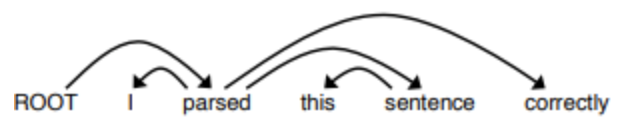
\includegraphics[width=0.3\textwidth]{4-1.png}
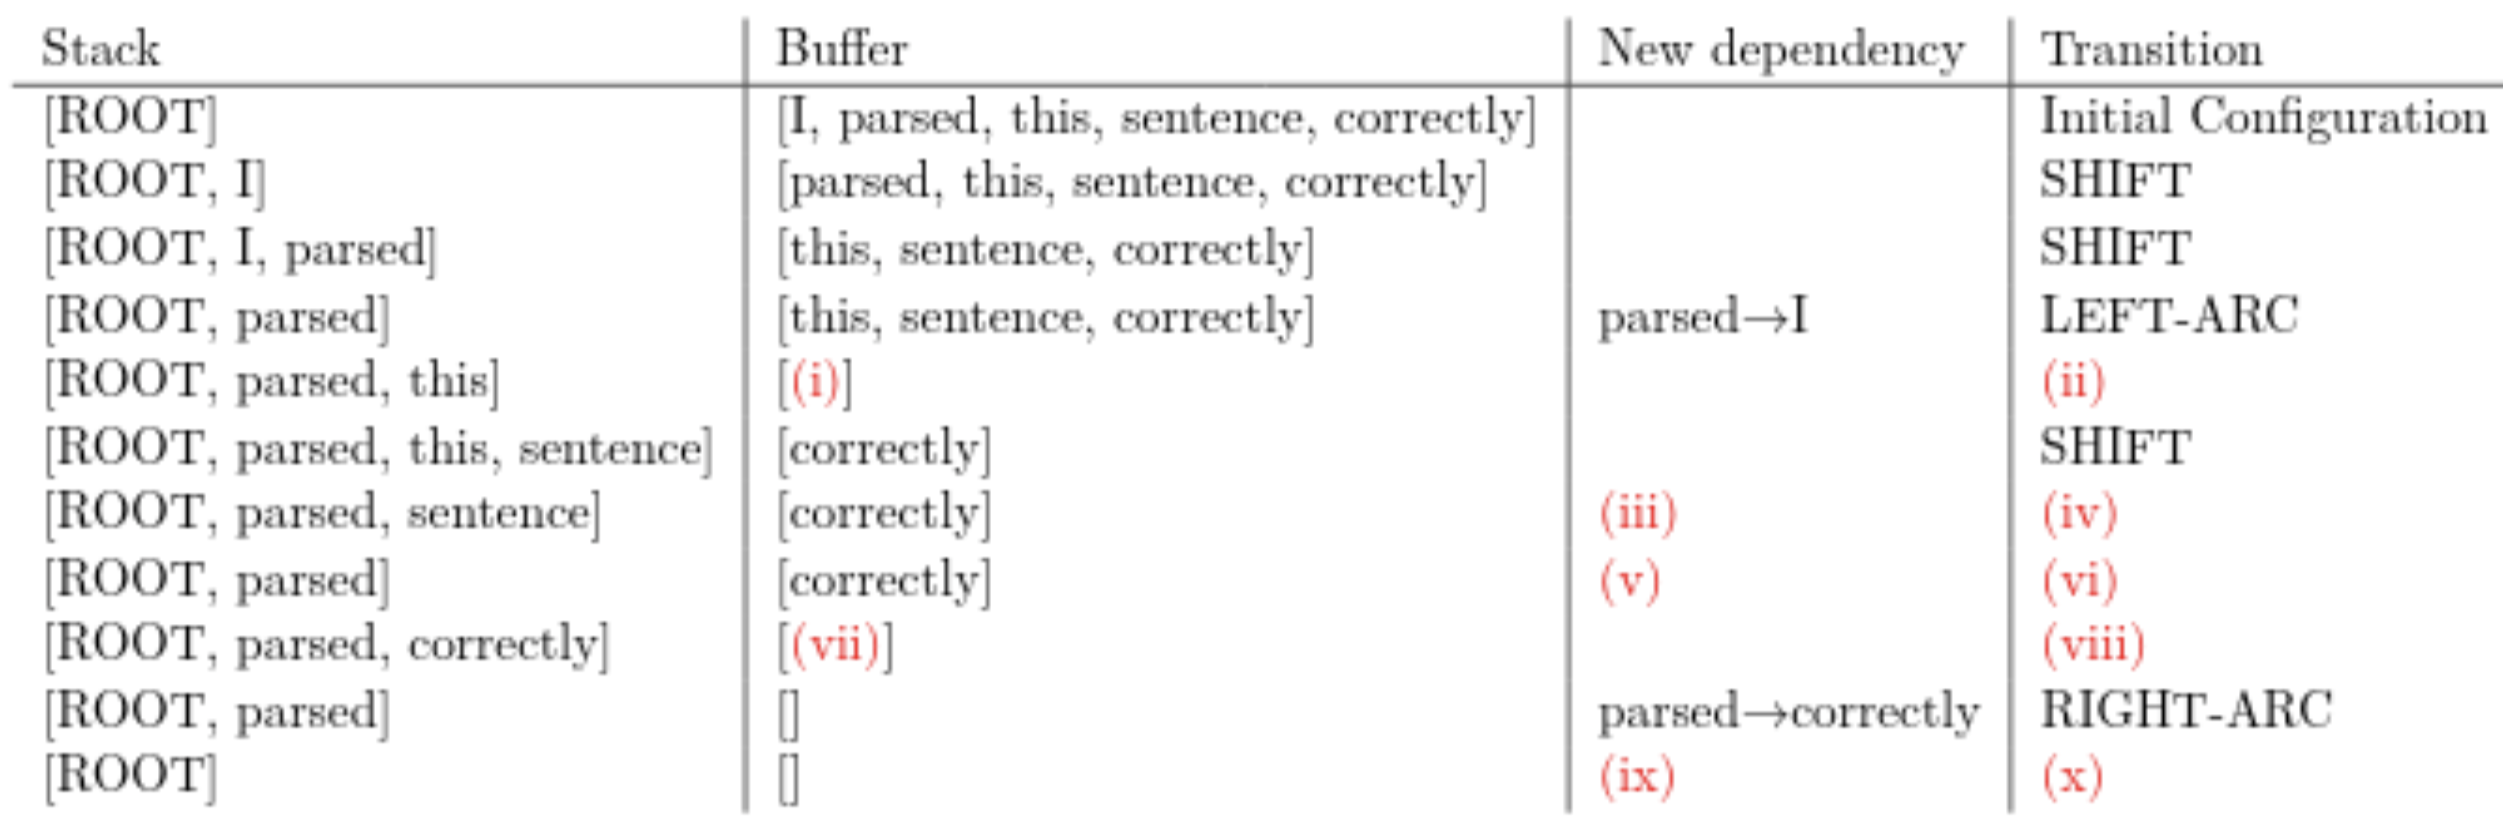
\includegraphics[width=0.75\textwidth]{4-2.png}
\end{center}

\begin{enumerate}[4a.]

\item \points{quiz4a} Select the right option for blanks (i) and (ii):

\begin{enumerate}[(a)]
\item (i) : [correctly]; (ii) SHIFT
\item (i) : [sentence, correctly]; (ii) SHIFT
\item (i) : parsed $\rightarrow$ this; (ii) LEFT-ARC
\item (i) : parsed $\rightarrow$ this; (ii) RIGHT-ARC
\end{enumerate}

% ### START CODE HERE ###
% ### END CODE HERE ###

\item \points{quiz4b} Select the right option for blanks (iii) and (iv):

\begin{enumerate}[(a)]
\item (iii) : leave it blank ; (iv) SHIFT
\item (iii) : sentence $\rightarrow$ correctly; (iv) LEFT-ARC
\item (iii) : sentence $\rightarrow$ this; (iv) LEFT-ARC
\item (iii) : sentence $\rightarrow$ this; (iv) RIGHT-ARC
\end{enumerate}

% ### START CODE HERE ###
% ### END CODE HERE ###

\item \points{quiz4c} Select the right option for blanks (v) and (vi):

\begin{enumerate}[(a)]
\item (v) : leave it blank ; (vi) SHIFT
\item (v) : sentence $\rightarrow$ correctly; (vi) LEFT-ARC
\item (v) : sentence $\rightarrow$ this; (vi) RIGHT-ARC
\item (v) : parsed $\rightarrow$ sentence; (vi) RIGHT-ARC
\end{enumerate}

% ### START CODE HERE ###
% ### END CODE HERE ###

\item \points{quiz4d} Select the right option for blanks (vii) and (viii):

\begin{enumerate}[(a)]
\item (vii) : [correctly] ; (viii) SHIFT
\item (vii) : []; (viii) : SHIFT
\item (vii) : parsed $\rightarrow$ correctly; (viii) LEFT-ARC
\item (vii) : parsed $\rightarrow$ correctly; (viii) RIGHT-ARC
\end{enumerate}

% ### START CODE HERE ###
% ### END CODE HERE ###

\item \points{quiz4e} Select the right option for blanks (ix) and (x):

\begin{enumerate}[(a)]
\item (ix) : ROOT $\rightarrow$ parsed; (x) RIGHT-ARC
\item (ix) : ROOT $\rightarrow$ parsed; (x) LEFT-ARC
\item (ix) : keep it blank; (x) SHIFT
\end{enumerate}

% ### START CODE HERE ###
% ### END CODE HERE ###

\end{enumerate}

\item \points{quiz5} A sentence containing $n$ words will be parsed in how many steps (in terms of $n$)?

\begin{enumerate}[(a)]
\item $2n$ steps
\item $n$ steps
\item $n^3$ steps
\item $0.5n$ steps
\end{enumerate}

% ### START CODE HERE ###
% ### END CODE HERE ###

{\bf Parsing Errors}

We'd like to look at example dependency parses and understand where parsers like ours might be wrong. For example, in this sentence:

\begin{center}
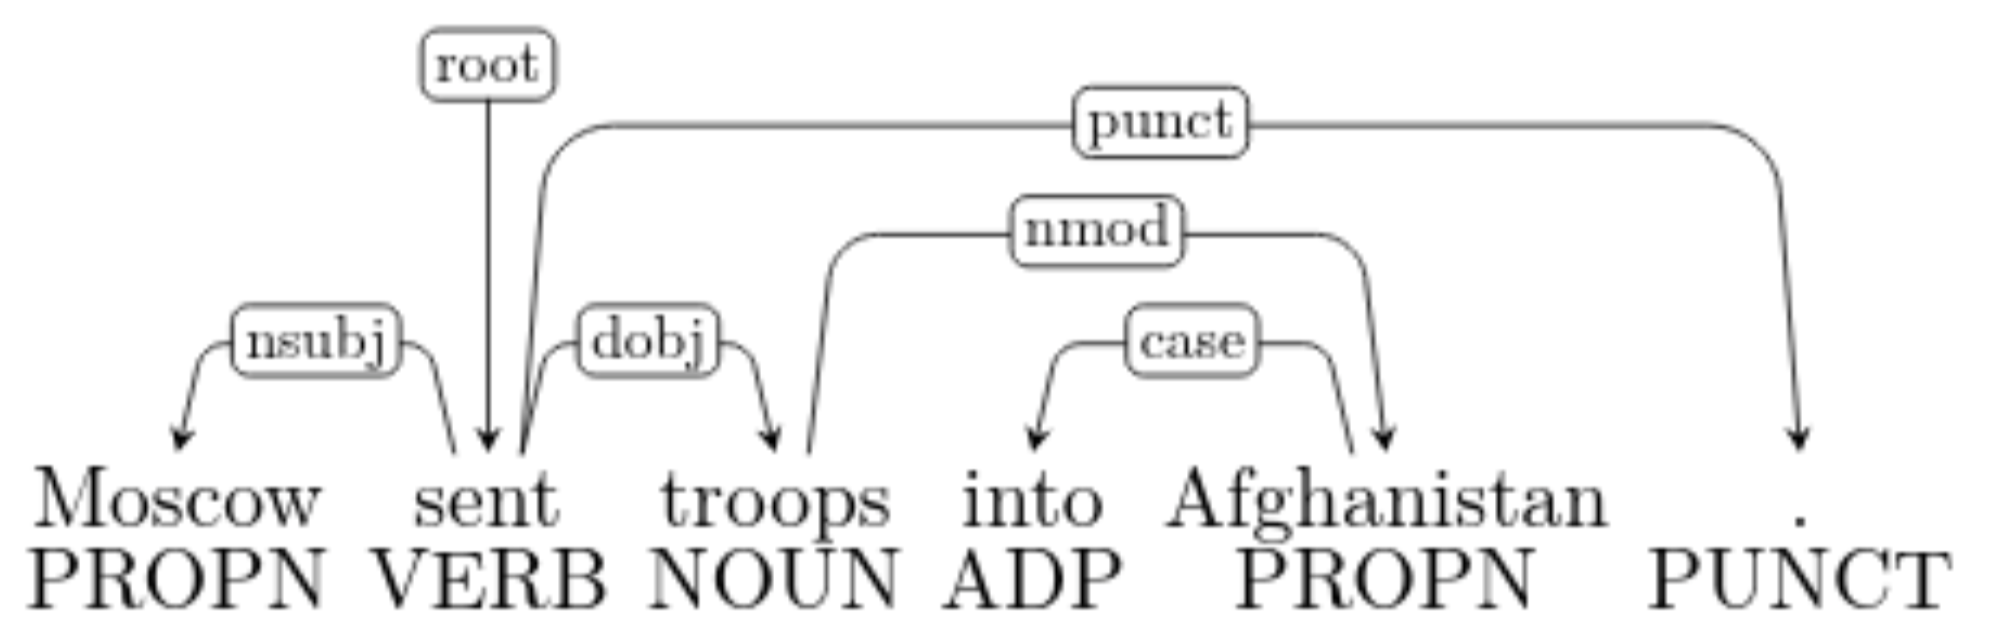
\includegraphics[width=0.75\textwidth]{6pre-1.png}
\end{center}

the dependency of the phrase {\bf into Afghanistan} is wrong because the phrase should modify {\bf sent} (as in {\em sent into Afghanistan}) not {\bf troops} (because {\em troops into Afghanistan} doesn't make sense). Here is the correct parse:

\begin{center}
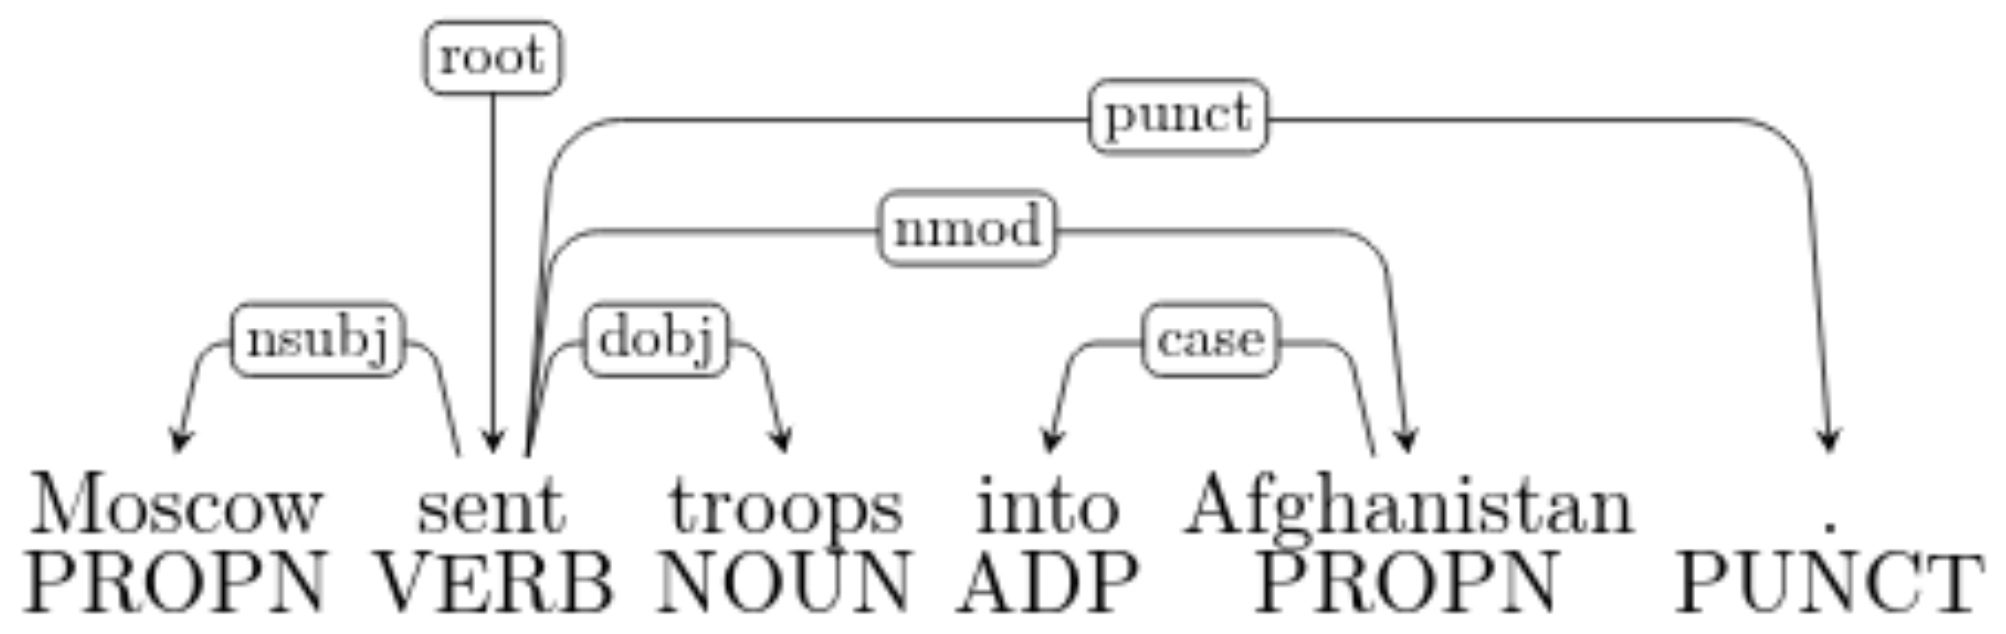
\includegraphics[width=0.75\textwidth]{6pre-2.png}
\end{center}

More generally, here are four types of parsing error:

\begin{itemize}
\item {\bf Prepositional Phrase Attachment Error:} In the example above, the phrase {\em into Afghanistan} is a prepositional phrase. A Prepositional Phrase Attachment Error is when a prepositional phrase is attached to the wrong head word (in this example, {\em troops} is the wrong head word and sent is the correct head word. More examples of prepositional phrases include {\em with a rock}, {\em before midnight} and {\em under the carpet}. 

\item {\bf Verb Phrase Attachment Error:} In the sentence {\em Leaving the store unattended, I went outside to watch the parade}, the phrase {\em leaving the store unattended} is a verb phrase. A Verb Phrase Attachment Error is when a verb phrase is attached to the wrong head word (in this example, the correct head word is {\em went}).
   
\item {\bf Modifier Attachment Error:} In the sentence, {\em I am extremely short}, the adverb {\em extremely} is a modifier of the adjective {\em short}. A Modifier Attachment Error is when a modifier is attached to the wrong head word (in this example, the correct head word is {\em short}).
 
\item {\bf Coordination Attachment Error:} In the sentence {\em Would you like brown rice or garlic naan}? the phrases {\em brown rice} and {\em garlic naan} are both conjuncts and the word or is the coordinating conjunction. The second conjunct (here {\em garlic naan}) should be attached to the first conjunct (here {\em brown rice}). A Coordination Attachment Error is when the second conjunct is attached to the wrong head word (in this example, the correct head word is {\em rice}). Other coordinating conjunctions include {\em and}, {\em but}, and {\em so}.
\end{itemize}

This question presents four sentences with dependency parses obtained from a parser. Each sentence has one error, and there is one example of each of the four types above. For each sentence, state the type of error, the incorrect dependency, and the correct dependency. To demonstrate: for the example above, you would write: 

\begin{itemize}
\item {\bf Error type:} Prepositional Phrase Attachment Error 
\item {\bf Incorrect dependency:} troops $\rightarrow$ Afghanistan 
\item {\bf Correct dependency:} sent $\rightarrow$ Afghanistan
\end{itemize}

{\em {\bf Note:}  There are lots of details and conventions for dependency annotation. If you want to learn more about them, you can look at the UD website: \url{http://universaldependencies.org}. However, you {\bf do not} need to know all these details in order to do these questions. In each of these cases, we are asking about the attachment of phrases and it should be sufficient to see if they are modifying the correct head. In particular, you {\bf do not} need to look at the labels on the dependency edges -- it suffices to just look at the edges themselves.}

For each sentence, select the correct combination of Error Type, Incorrect Dependency, and Correct Dependency.

\item \points{quiz6}

\begin{center}
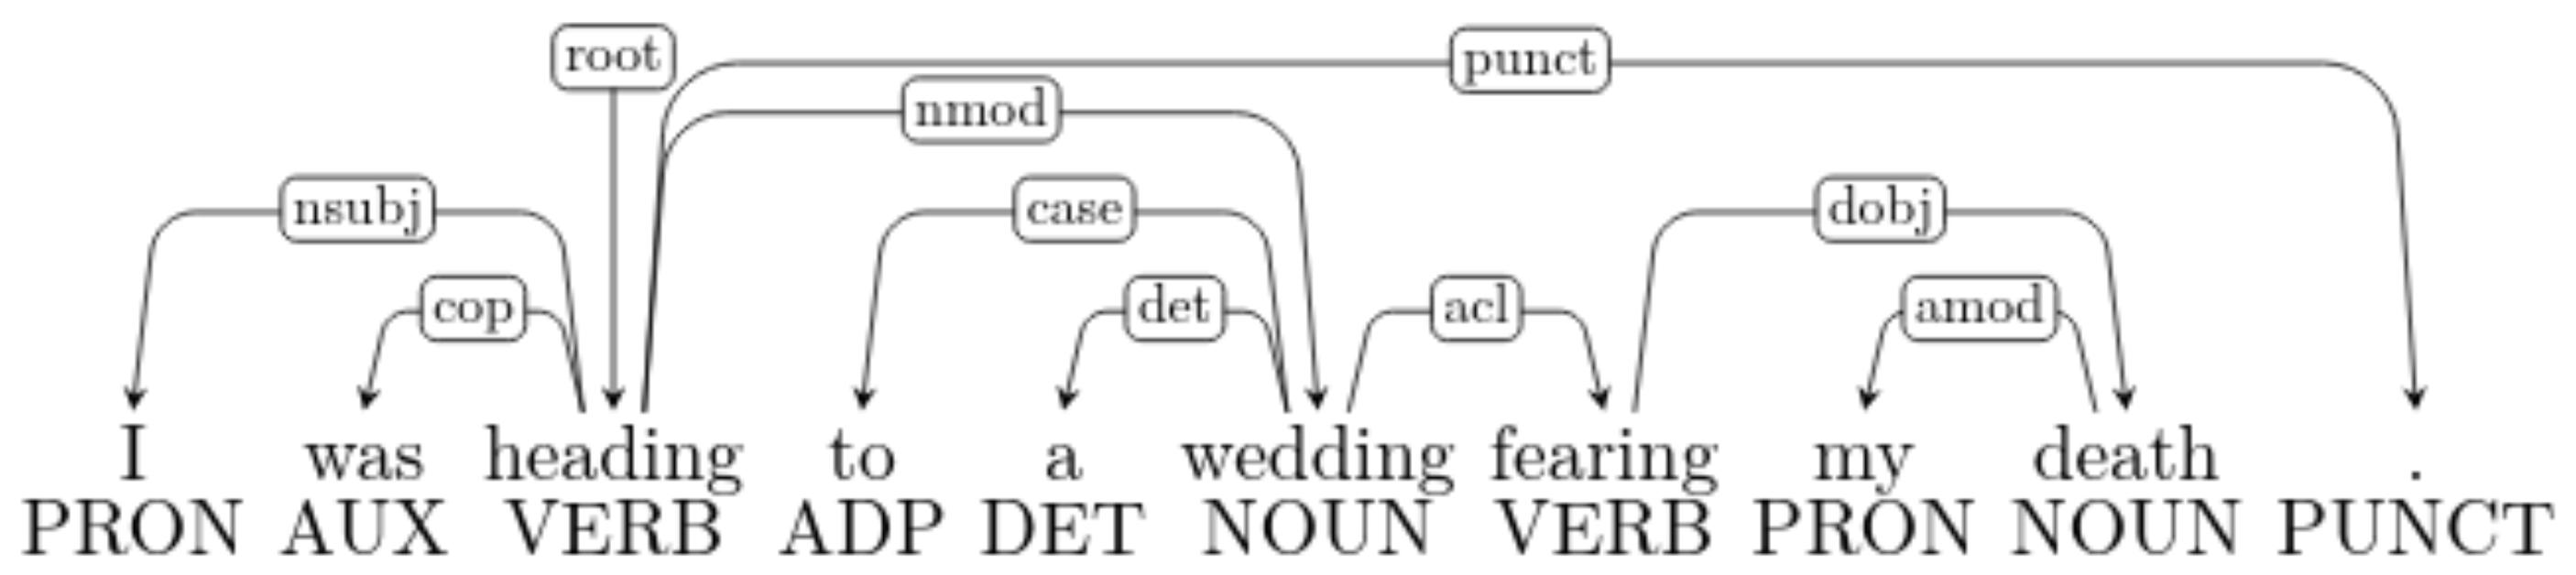
\includegraphics[width=0.75\textwidth]{6-1.png}
\end{center}

\begin{enumerate}[(a)]
\item {\bf Error type:} Verb Phrase Attachment Error

{\bf Incorrect dependency:} wedding $\rightarrow$ fearing

{\bf Correct dependency:} I $\rightarrow$ fearing

\item {\bf Error type:} Prepositional Phrase Attachment Error

{\bf Incorrect dependency:} wedding $\rightarrow$ fearing

{\bf Correct dependency:} I $\rightarrow$ death

\item {\bf Error type:} Verb Phrase Attachment Error

{\bf Incorrect dependency:} wedding $\rightarrow$ fearing

{\bf Correct dependency:} heading $\rightarrow$ I

\item {\bf Error type:} Coordination Attachment Error

{\bf Incorrect dependency:} wedding $\rightarrow$ fearing

{\bf Correct dependency:} heading $\rightarrow$ death OR I $\rightarrow$ death

\end{enumerate}

% ### START CODE HERE ###
% ### END CODE HERE ###

\item \points{quiz7}

\begin{center}
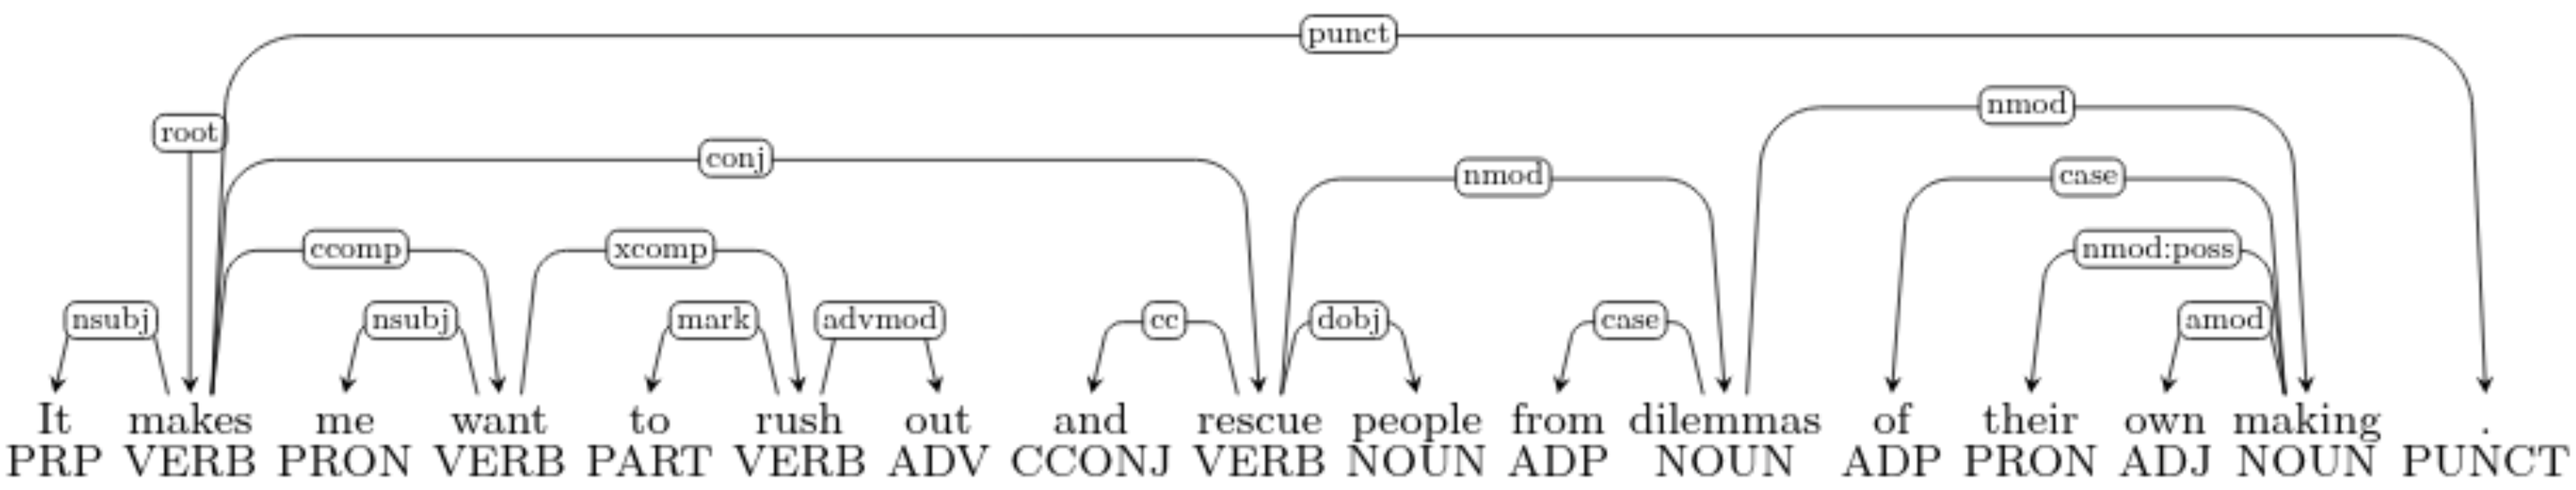
\includegraphics[width=0.75\textwidth]{7-1.png}
\end{center}

\begin{enumerate}[(a)]
\item {\bf Error type:} Prepositional Phrase Attachment Error

{\bf Incorrect dependency:} makes $\rightarrow$ rescue 

{\bf Correct dependency:} rush $\rightarrow$ dilemma

\item {\bf Error type:} Modifier Attachment Error

{\bf Incorrect dependency:} makes $\rightarrow$ rescue

{\bf Correct dependency:} want $\rightarrow$ rescue

\item {\bf Error type:} Coordination Attachment Error 

{\bf Incorrect dependency:} makes $\rightarrow$ rescue 

{\bf Correct dependency:} rush $\rightarrow$ rescue

\item {\bf Error type:} Verb Phrase Attachment Error

{\bf Incorrect dependency:} makes $\rightarrow$ rescue

{\bf Correct dependency:} want $\rightarrow$ rush

\end{enumerate}

% ### START CODE HERE ###
% ### END CODE HERE ###

\item \points{quiz8}

\begin{center}
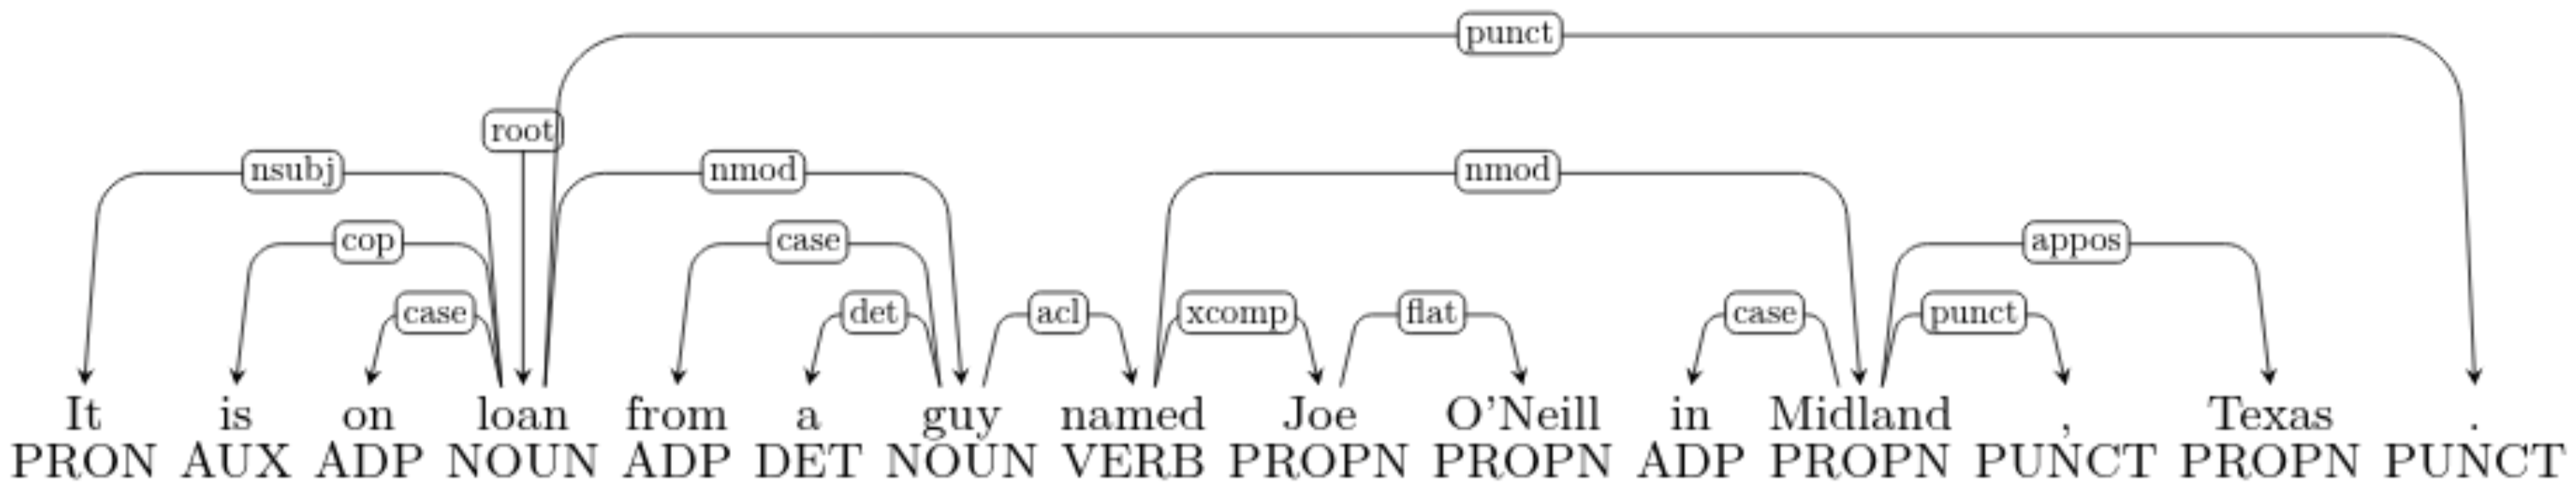
\includegraphics[width=0.75\textwidth]{8-1.png}
\end{center}

\begin{enumerate}[(a)]
\item {\bf Error type:} Coordination Attachment Error

{\bf Incorrect dependency:} named $\rightarrow$ Midland 

{\bf Correct dependency:} joe $\rightarrow$ Midland

\item {\bf Error type:} Modifier Attachment Error

{\bf Incorrect dependency:} named $\rightarrow$ Midland

{\bf Correct dependency:} loan $\rightarrow$ joe

\item {\bf Error type:} Prepositional Phrase Attachment Error 

{\bf Incorrect dependency:} named $\rightarrow$ Midland 

{\bf Correct dependency:} guy $\rightarrow$ Midland

\item {\bf Error type:} Verb Phrase Attachment Error

{\bf Incorrect dependency:} named $\rightarrow$ Midland

{\bf Correct dependency:} loan $\rightarrow$ Midland

\end{enumerate}

% ### START CODE HERE ###
% ### END CODE HERE ###

\item \points{quiz9}

\begin{center}
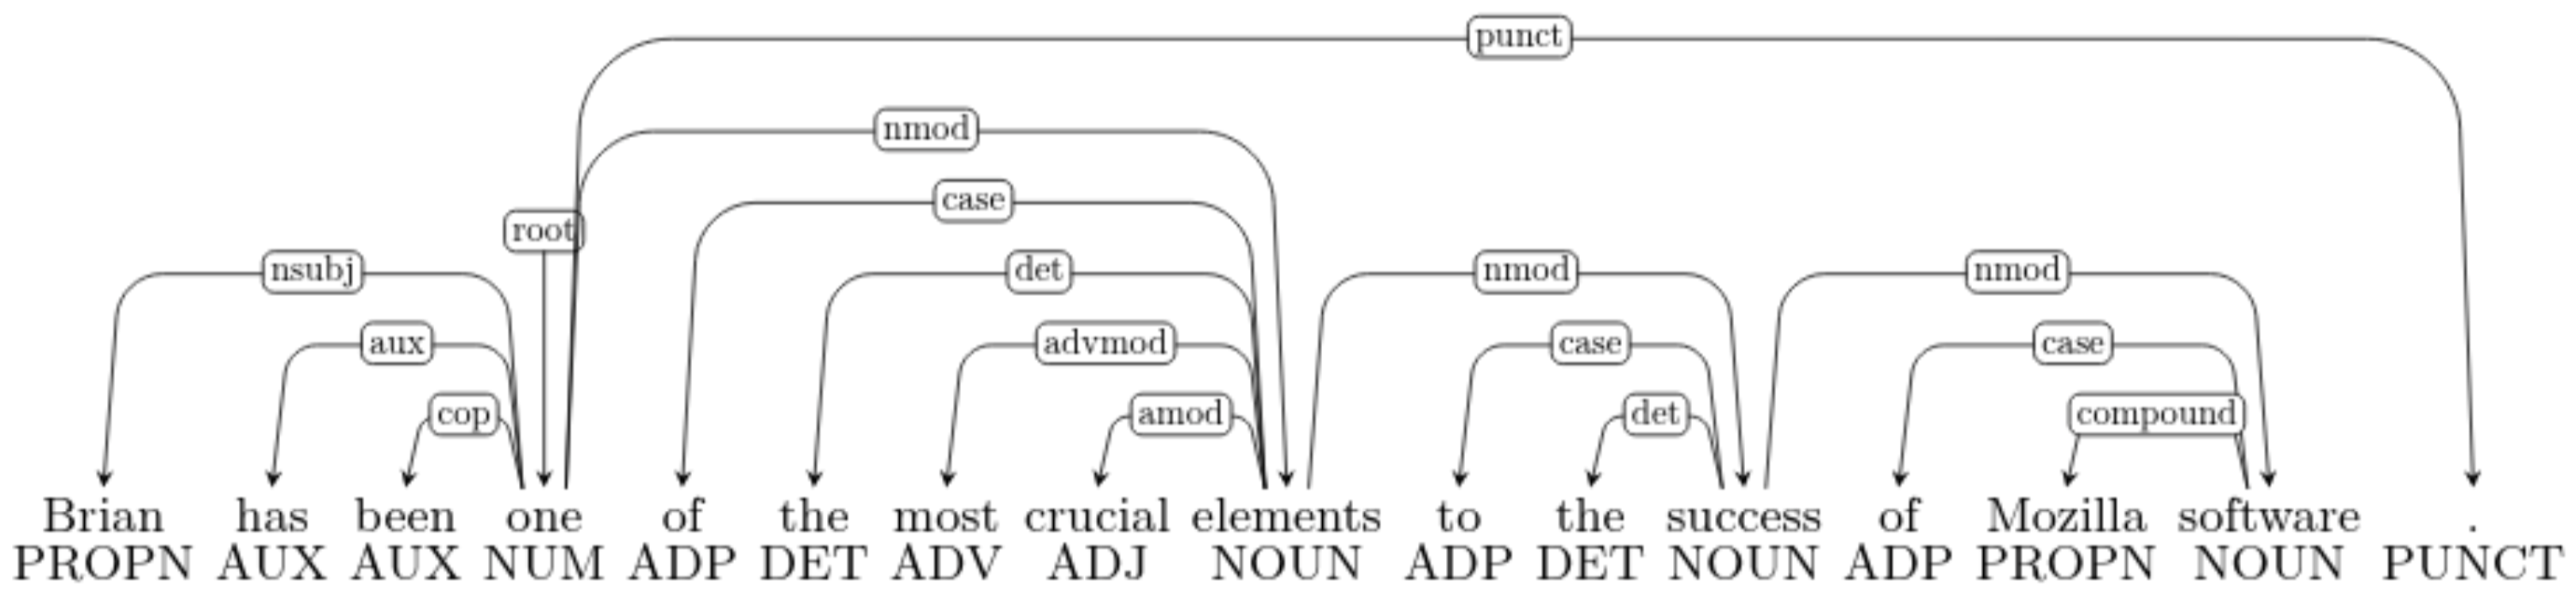
\includegraphics[width=0.75\textwidth]{9-1.png}
\end{center}

\begin{enumerate}[(a)]
\item {\bf Error type:} Coordination Attachment Error

{\bf Incorrect dependency:} elements $\rightarrow$ most 

{\bf Correct dependency:} elements $\rightarrow$ software

\item {\bf Error type:} Modifier Attachment Error 

{\bf Incorrect dependency:} elements $\rightarrow$ most 

{\bf Correct dependency:} crucial $\rightarrow$ most

\item {\bf Error type:} Prepositional Phrase Attachment Error

{\bf Incorrect dependency:} elements $\rightarrow$ most

{\bf Correct dependency:} one $\rightarrow$ success

\item {\bf Error type:} Verb Phrase Attachment Error

{\bf Incorrect dependency:} elements $\rightarrow$ most

{\bf Correct dependency:} one $\rightarrow$ software

\end{enumerate}

% ### START CODE HERE ###
% ### END CODE HERE ###

\end{enumerate}